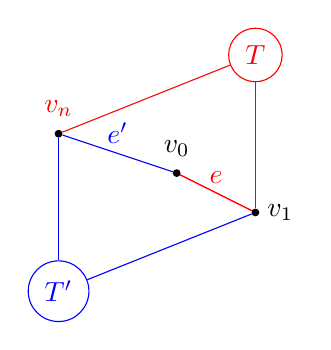
\begin{tikzpicture}[node distance=9pt]
\tikzstyle{blackdot}=[circle,scale=0.3,fill];

\draw[draw=red] (0,-0.5) node [blackdot] (v0) {} -- (1,-1)node [blackdot] (v1) {};
\node[above of=v0] {$v_0$};
\node[right of=v1] {$v_1$};
\node[draw,circle,minimum width=16pt,red] (v2) at (1,1) {$T$};
\draw[red]  (v2) edge (v1);
\draw[red]  (v0) edge node[above] {$e$} (v1);
\draw (-1.5,0) node[blackdot] (vn) {} edge[dashed,draw=none] (v0);
\node[above of=vn,red] {$v_n$};

%\draw[dashed,blue]  plot[smooth, tension=.7] coordinates {(v1) (0.5,-2.5) (-2,-2.5) (-2.5,-1) (vn)};
\draw[red]  (vn) edge (v2);
\draw[blue]  (vn) edge[draw=none] node[above] {$e^\prime$} (v0);
\node[draw,circle,minimum width=16pt,blue] (v2) at (-1.5,-2) {$T^\prime$};
\draw[blue]  (v2) edge (vn);
\draw[blue]  (v2) edge (v1);
\draw[blue]  (v0) edge (vn);
\end{tikzpicture}
